\lstdefinestyle{mystyle}{
    backgroundcolor=\color{myyellow},
    basicstyle=\ttfamily\small,
    breaklines=true,
    frame=single,
    language=XML
}

\chapter{State-of-the-Art Analysis} \label{ch:state-of-the-ArtAnalysis}
The following chapter constitutes an in-depth exploration of current technologies and methodologies within the automotive industry, with a specific focus on the complexity of vehicular software development. Firstly, the current automotive landscape will be examined, providing a detailed insight into challenges associated with software development in vehicles.

Subsequently, through meticulous analysis of scientific publications, technical reports, and practical implementations, the chapter delves into the radical transformation of the automotive sector facilitated by the concept of Software Defined Vehicle (SDV). This technology, crucial for technological progress and vehicular safety, will be explored from various perspectives. Particularly, the synergy between Cloud, software, and hardware will be investigated, highlighting solutions proposed by major industry players and analyzing their applications, benefits, and limitations.

The objective is to offer a comprehensive overview of current dynamics, emphasizing the pivotal role of SDV in the evolution of the automotive industry.

\section{Current Automotive Software Development}

In the past, the automotive industry advanced primarily through the development of technologies in mechanical engineering, focusing on perfecting combustion engines. Nowadays, the paradigm has radically changed due to multiple factors, including electrification, automation, shared mobility, and connected mobility.

Software technology development in the automotive field can be metaphorically compared to what has happened in smartphone development, as highlighted in the manifesto document regarding Bosch's Software Defined Vehicle (SDV) \cite{SDVBoschMobility}.

The ultimate goal is to achieve simple and user-friendly devices that fully meet the user's needs. Currently, many customers express dissatisfaction because their cars do not offer the same functionality and ease of use common in smartphones. Many ask: Why can't my \$50,000 car perform the same tasks as my \$300 smartphone?

A key difference between the automotive and smartphone industries is the level of complexity, which brings with it a number of issues.

\subsection{difficulties}
We can analyse in depth the problems of the current automotive software that is being developed via 4 main difficulties:

\begin{itemize}
    \item \textbf{Specialized Hardware:} Today's vehicles are still complex systems of systems. Each subsystem in a car, from brakes to transmission, is a complex entity, supplied by a different manufacturer and integrated with a unique software architecture. The level of complexity and the need for seamless interoperability between systems far exceeds that of today's smartphones.
    \item \textbf{Time:} The software production pipeline involves many development and testing steps with a not inconsiderable amount of time spent on each one. This is greatly increased by the presence of different components, so development time must be considered for each different unit of the system.
    \item \textbf{Cost:} The complexity of the software systems in vehicles entails very high costs, aggravated by the fact that the test phase is often carried out directly on the boards (for hardware requirements), which means a much longer production process, especially in the event of errors.
    
    \begin{figure}[h]  % 'h' significa che la figura viene posizionata qui
        \centering
        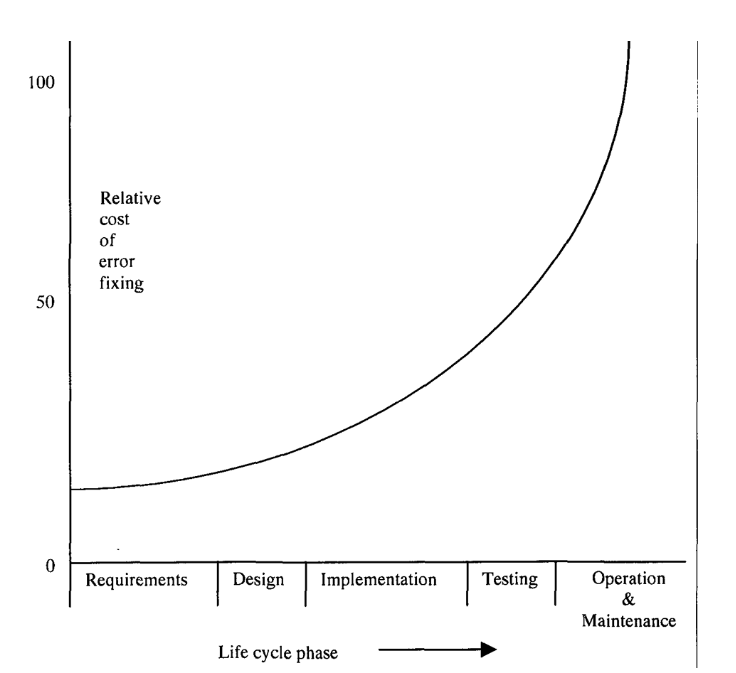
\includegraphics[width=0.9\textwidth]{images/costs_of_errors_correction_in_software_development.png}  % Sostituisci 'nome_immagine' con il nome del tuo file immagine e l'estensione
        \caption{Cost of fixing errors increases in later phases of the life cycle \cite{CostsOfSoftwareDeveloping}}
        \label{fig:WorldAutomobileProduction}
      \end{figure}

    \item \textbf{Human Safety Security:} Automotive embedded software must meet stringent reliability and security requirements, while delivering performance and a reasonable memory footprint. To develop automotive embedded software, you need the right tools that meet safety and security standards to evaluate, prototype and test your software.
\end{itemize}

What lessons can be drawn from the study of barriers that can be applied to the vehicle lifecycle? Historically, the vehicle lifecycle has been characterised by the simultaneous production and deployment of tightly integrated hardware and software. Once the vehicle was in the hands of the consumer, its characteristics remained largely unchanged until the end of its life. However, the SDV paradigm introduces the possibility of decoupling hardware and software release dates, a prerequisite for adopting a digital-first approach. This approach brings the design and virtual validation of the digital vehicle experience to the forefront of the lifecycle.
It also requires the application of the digital-first concept, which means that new ideas for the vehicle experience are first explored in virtual environments to ensure early user feedback, long before any custom hardware needs to be developed or a physical test vehicle is available. Digital first is the application of design thinking and lean startup principles, originally rooted in internet culture, to the tangible realm of automotive development.

%“Automakers and their suppliers need to continuously review and improve the testing approach in design and development, as well as look for new tools that automate and increase test coverage of their products,” Giallorenzo explained. “Cloud emulation is a major innovation that is coming to the industry to facilitate development and testing. Historically, testing of embedded software solutions has been hindered by the lack of chipsets and hardware, which is required to properly test complete hardware-plus-software solutions. This was particularly painful during the recent COVID-induced supply chain crunch."

\section{Introduction to Software Defined Vehicle}
The Software Defined Vehicle represents the new frontier of automotive manufacturing and is poised to completely change the paradigm of automotive production. 

If we imagine bringing a feature update to one of today's vehicles, it will most likely take anywhere from one to seven years from the idea to when that feature is actually perceptible in the production vehicle; this takes so long because the vehicles produced up to this point have not been designed with frequent updates in mind \cite{SDVBosch}.
Traditionally focused on physical functionality, the automotive industry has evolved from early electronic features such as airbags, vehicle stabilisation and braking systems to modern driver assistance and even automated driving. 
The current shift towards a digital experience is possible thanks to vehicle design that includes software integration as a fundamental part. Software should no longer be seen as an accessory to the vehicle, but as an integral part of the vehicle itself.

The simultaneous efforts of major automotive companies such as Bosch, Renault and Stellantis, in collaboration with leading computer developers such as Arm, BlackBerry and AWS, have given rise to the Software Defined Vehicle concept, which they define as "any vehicle that manages its own operations, adds functionality and enables new features primarily or entirely through software" \cite{blackberrySDV}.

It is evident that the Software Defined Vehicle represents the future of the automotive industry, promising an enriched and enduring user experience, coupled with the evolution of automotive technologies. This section further elucidates the current state of the industry, highlighting the key players that are working in the industry as a enablers to develop the SDV technologies, and  the benefits of this innovation.

\subsection{Enablers}
The software defined vehicle solution is nowadays being considered by several companies as the manifesto of a new era of vehicle development. An example is given by the renault group, which in an overview of its products describes: "Today, it is already possible to make remote updates of some vehicles via the Firmware Over The Air (FOTA) system. This keeps the vehicle safe by making it easier and faster to improve the on-board system and apply patches. Tomorrow, the Software Defined Vehicle's flexible and scalable architecture will enable the faster development and integration of new features throughout the vehicle lifecycle, directly into the cloud, that is, in secure online servers accessible from anywhere and anytime" \cite{SDVRenault}. 

Two key technology players, Arm and AWS, have played a pivotal role in advancing SDV by working together to define standards that accelerate technology development.
\begin{itemize}
    \item \textbf{Arm:} a leading semiconductor design and software company, is a pillar in the advancement of SDV technology. Focusing on the development of energy-efficient processors and technologies, Arm's contributions enable SDVs to efficiently manage their operations, add functionality and introduce new features through the development of general-purpose processors that can be used in the cloud for software development and maintenance, and in the vehicle itself to maintain computing continuity.
    \item \textbf{Amazon Web Services (AWS):} a global leader in cloud computing, offers scalable and secure solutions for real-time application updates, enhanced connectivity, and efficient data management. The AWS services and technologies will be in depth described in the futher chapters.
\end{itemize}

The collaborative efforts of this two companies contribute to shaping a future where vehicles are not only defined by their physical attributes but are also dynamic entities capable of continual software-driven enhancements and innovations.

\subsection{Benefits}
The Software Defined Vehicle, as introduced in the previous chapters, brings several benefits to both automotive companies and the end-user experience.  These innovations are made possible by the fact that the vehicle becomes a device that can be constantly monitored and updated in real time via the cloud throughout its entire lifecycle. Let us now look at the key benefits.

From the point of view of this project, the main innovation brought by this technology is the security of the device software. Since, as mentioned above \cite{ISO26262}, vehicles are considered as safety elements critical to human life, the safety benefits can be analysed from two perspectives:
\begin{itemize}
    \item \textbf{Human Safety Critical Security:} The ability of SDV to receive real-time data from the vehicle allows in-depth monitoring of all its components. Taking the influence of tyres as an example, it has been found that most road accidents are caused by tyre wear and lack of regular maintenance. It is therefore necessary to assess the health of tyres through continuous monitoring of physical parameters such as tyre thickness, temperature and pressure, as well as regular maintenance. This helps to eliminate or minimise the possibility of tyre bursts and subsequent accidents. It also improves the safety of people and vehicles \cite{PredictDefectsOfTiresInHeavyVehicle}. These factors can be monitored either manually or automatically: manual predictive maintenance requires human intervention and can lead to some errors; automatic predictive maintenance using artificial intelligence can be more efficient \cite{AirPressureSystemFailurePrediction}. Renault defines this work as "predictive maintenance" \cite{SDVRenault}, stressing the importance of collecting and analysing data in a centralised system to anticipate and prevent potential failures, ensure the safety of people, reduce maintenance costs and improve the performance of the vehicle.
    \item \textbf{Intrinsic Software Security:} In the presence of bugs and vulnerabilities in the vehicle's software, SDV makes it possible to intervene promptly to resolve each problem and reduce the window of exposure.
    \begin{figure}[h]  % 'h' significa che la figura viene posizionata qui
        \centering
        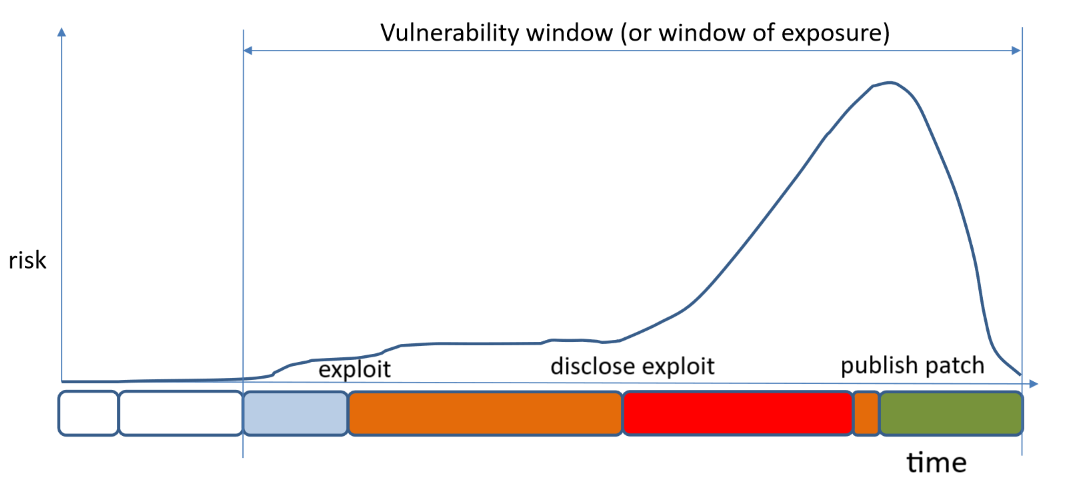
\includegraphics[width=0.8\textwidth]{images/window_of_exposure.png}  % Sostituisci 'nome_immagine' con il nome del tuo file immagine e l'estensione
        \caption{Risks and time relationship in the various phases of a vulnerability lifecycle}
        \label{fig:WindowOfExposure}
    \end{figure}

    A crucial aspect of vehicle software security is the robustness of the algorithms, especially in the context of autonomous driving. In this context, a predictive algorithm responsible for vehicle safety decisions can be continuously improved and optimised. The SDV also introduces the concept of the 'digital twin', a platform that virtually replicates the functionality and behaviour of the vehicle. Thanks to this technology, predictive algorithms used in autonomous driving can be effectively tested on the cloud platform and, when ready, integrated directly into the vehicle.
\end{itemize}

From a user experience point of view, two other significant benefits can be identified: an increase in the value of the vehicle, which can be continuously upgraded over time, and the ability to enable additional vehicle functions via software. For example, the user can decide to activate a feature for a certain period of time and then deactivate it (paying only for the time it is used), or activate a new feature that was not available at the time of purchase. In essence, the vehicle becomes a dynamic platform that is constantly evolving and fully customisable through the software.

For automotive companies, the benefits mentioned so far can bring direct benefits to the industry. In support of this, Stellantis reports that: "the team in Poland will contribute to the global software creation network that is key to Stellantis' work in creating software-defined vehicles (SDVs) that offer customer-focused features throughout the vehicle's life span, including updates and features that will be added years after the vehicle is manufactured. “Creating an infrastructure inside our vehicles that easily and seamlessly adapts to meet driver expectations is a key element of Stellantis' global drive to deliver cutting edge mobility. Stellantis' software-driven strategy deploys next-generation tech platforms, building on existing connected vehicle capabilities to transform how customers interact with their vehicles and to generate €20 billion in incremental annual revenues by 2030".

In addition, the SDV paradigm brings an advantage from a software production pipeline perspective. In today's software production scenario, there can be two development mechanisms:
\begin{itemize}
    \item A more traditional mode in which software is created directly on the system, hence on the processor itself. This is undoubtedly the most inconvenient solution, as it would require unnecessary overuse of processors, wasting resources, money and time.
    \item Alternatively, developers rely on cumbersome operating system emulation tools on the host machine and the cross-compilation process, which uses a dedicated compiler to produce executable code for the target system. Once the code is on the development system, a final integration and validation test can be performed, but scalability is limited to the number of physical hardware platforms. 
\end{itemize}

Typical workflows for the development, integration and validation of embedded systems are as follows \cite{DevelopersWorkflow}:
\begin{figure}[h]  % 'h' significa che la figura viene posizionata qui
    \centering
    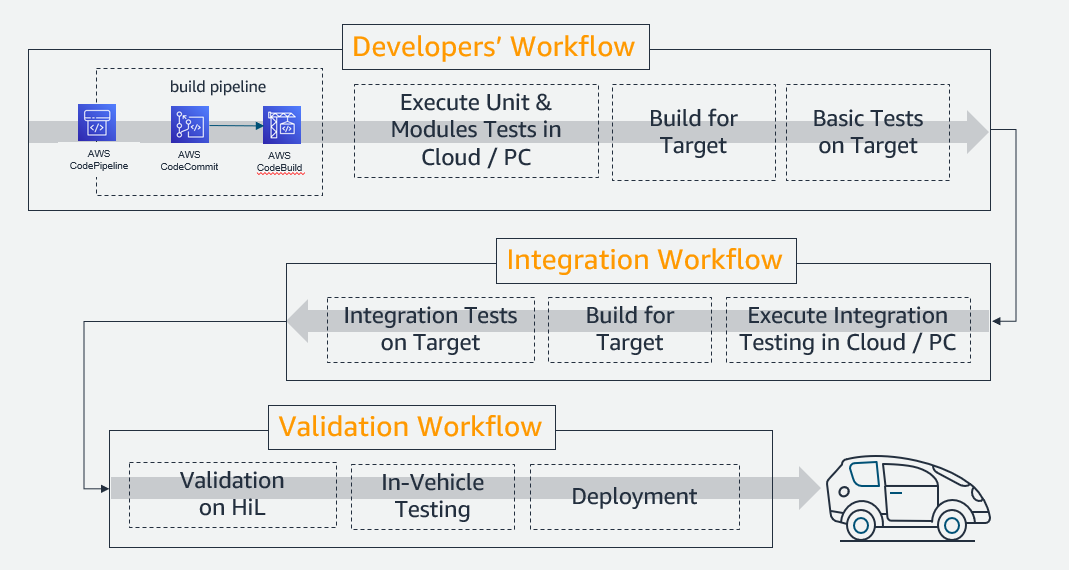
\includegraphics[width=0.7\textwidth]{images/today_developer_workflow.png}  % Sostituisci 'nome_immagine' con il nome del tuo file immagine e l'estensione
    \caption{today development, integration, and validation workflows for embedded systems}
    \label{fig:TodayDeveloperWorkflow}
\end{figure}

As explained in the following chapters, by using the software defined vehicle, i.e. operating systems that rely on general purpose porpouse architectures to provide parity between cloud and edge systems, it is possible to reduce the embedded developer's workflow to remove many of the steps that are now no longer required, as shown in the diagram below \cite{DevelopersWorkflow}:
\begin{figure}[h]  % 'h' significa che la figura viene posizionata qui
    \centering
    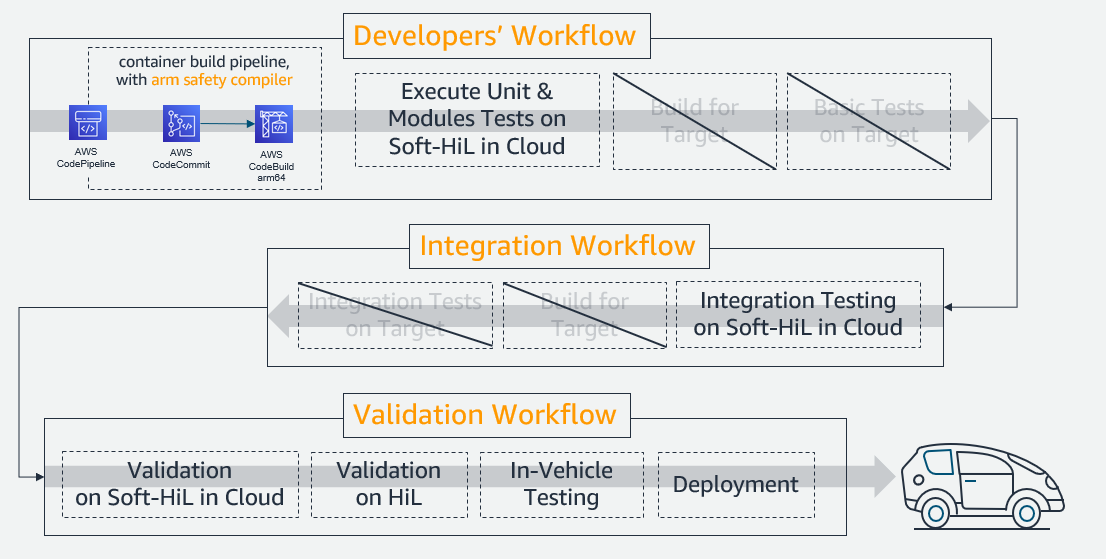
\includegraphics[width=0.7\textwidth]{images/future_developers_workflow.png}  % Sostituisci 'nome_immagine' con il nome del tuo file immagine e l'estensione
    \caption{future development, integration, and validation workflows for embedded systems}
    \label{fig:FutureDevelopersWorkflow}
\end{figure}

\subsection{initiatives}
(ARCHITETTURA DEL SDV CON RIFERIMENTO A ARM E AWS SOAFEE )
